% dye_table_mileposts.tex
% by Troy Hix, May 2005
%----------------------------------------------------------------------------
\begin{sidewaysfigure}
\center
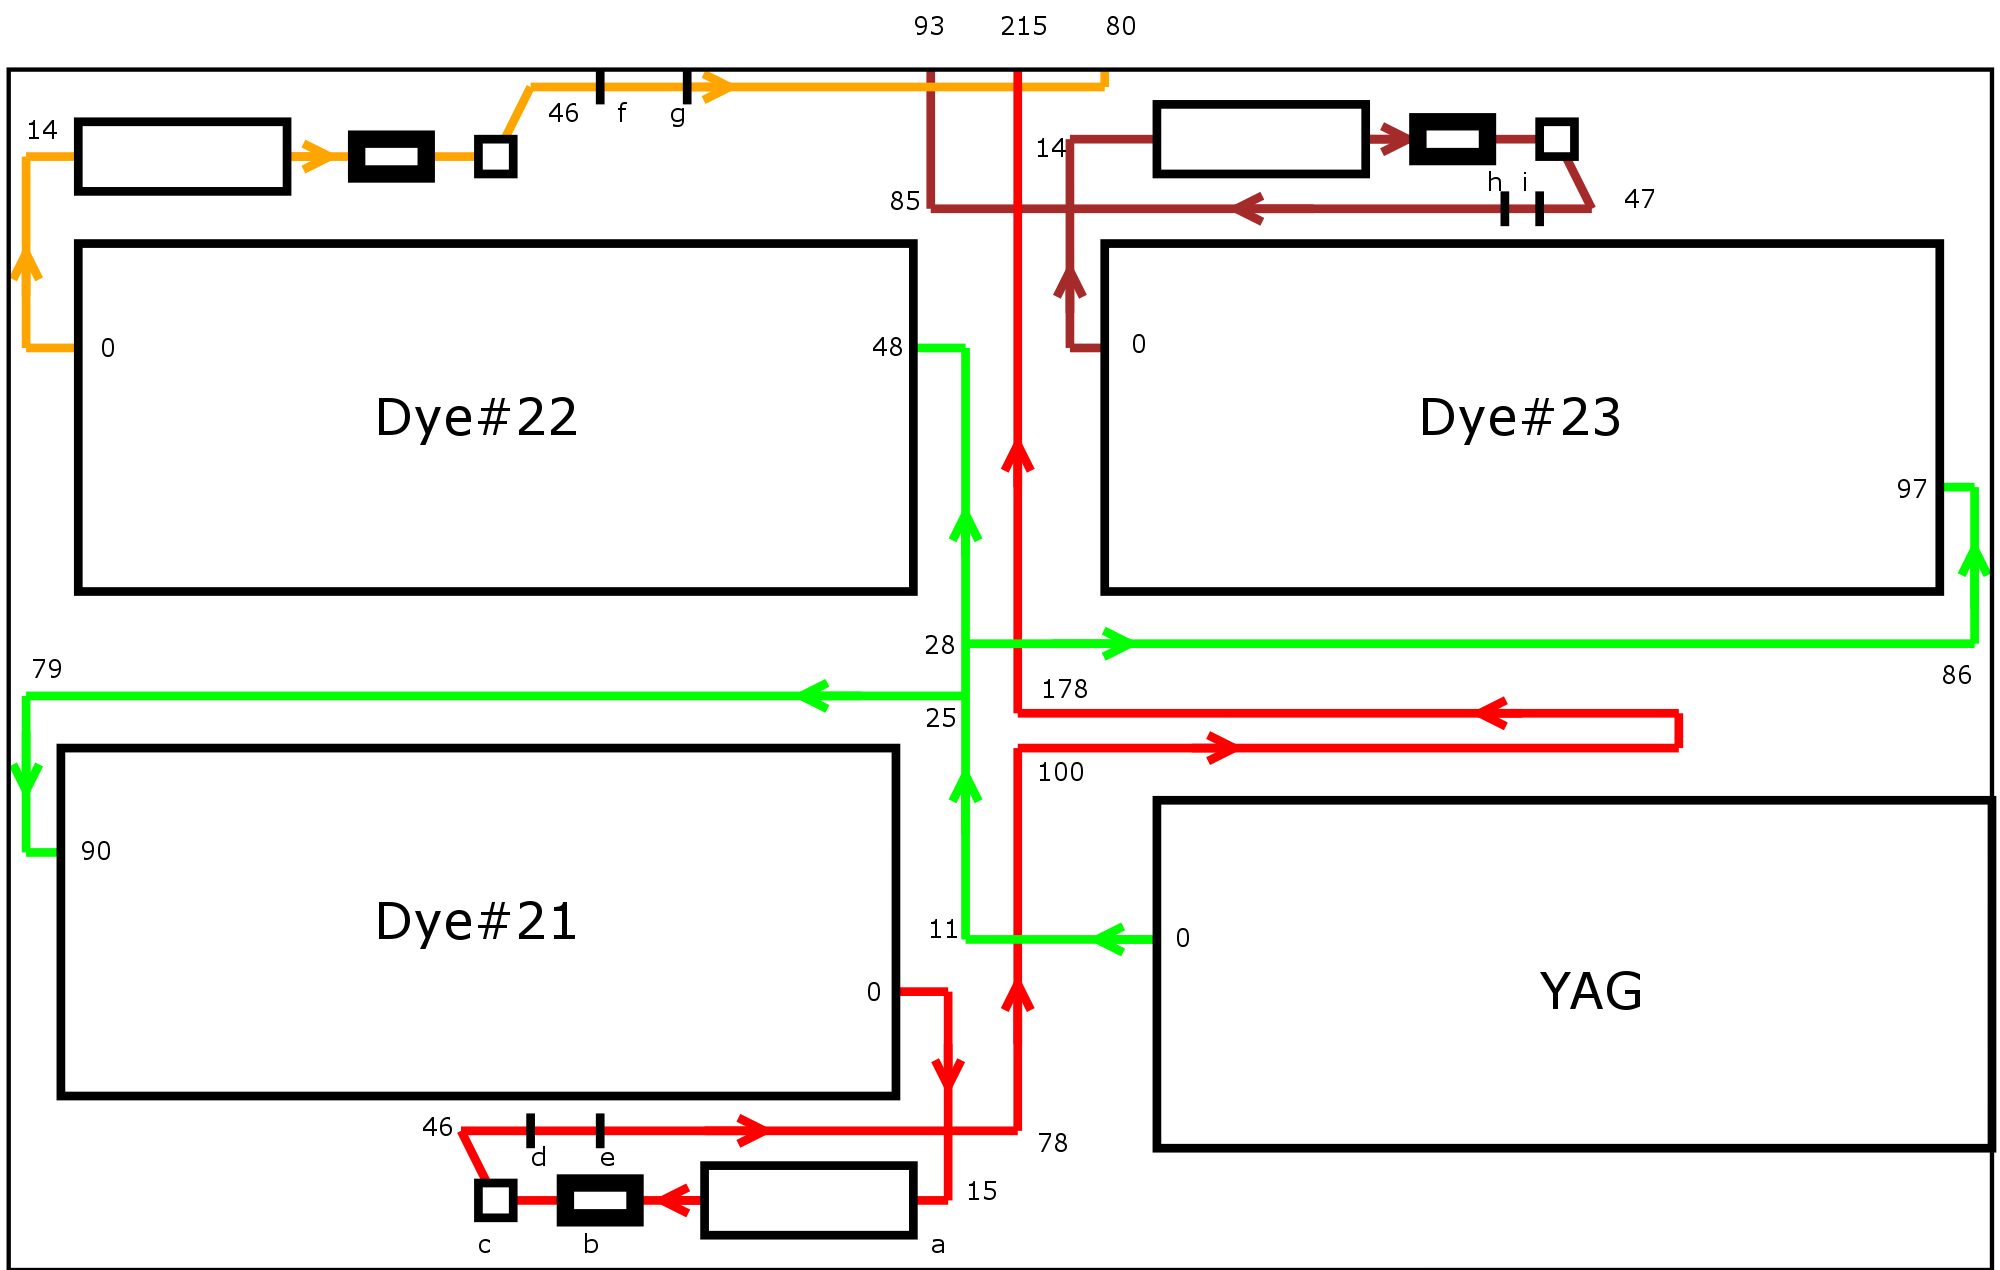
\includegraphics[width=7.75in]
{dye_mileposts/dye_mileposts.png}
\caption[Beam mileposts and optics on the dye laser table]{Beam mileposts and optics on the dye laser table. the mileposts along each beam line is given in inches. Optic (a) is a pile-of-plates polarizer; (b) Pockels cell, (c) Brewster plate, (d) +1 m lens at mile post 50, (e) -1 m lens at milepost 54, (f) +1 m lens at milepost 50, (g) -1 m lens at milepost 55, (h) +1 m lens at milepost 50, (i) -1 m lens at milepost 52.5.}
\label{dye_mileposts}
\end{sidewaysfigure} 
%----------------------------------------------------------------------------
%----------------------------------------------------------------------------
%----------------------------------------------------------------------------


